\section{Performance Evaluation}

In this section, we show that:

\begin{itemize}

\item In the network with fixed bandwidth, compared with state-of-the-art VR streaming system, PQVRS saves 45\% bandwidth on average while providing the same PSPNR, or provides 15-20 higher PSPNR in the same bandwidth.

\item In the network with unstable bandwidth, PQVRS improves 10 higher PSPNR and decreases up to 50\% stalling.

\item In real-world perceived quality rating by users, PQVRS can obtain notable higher user rating.

\item PQVRS introduce less CPU workload than state-of-art VR streaming system.

\end{itemize}

\subsection{Evaluation Setup}

Our evaluation consists of a large-scale trace-driven simulation and a small scale real-world end-to-end experiment.

\subsubsection{Trace-driven simulation}
~\\

\textbf{Video: } There are 50 videos in our simulation, with each video 5min on average. Among these 50 videos, 18 of them are obtained from \cite{VRdataset} and the other 32 are collected from IQiYi [?]. All videos are in 2880*1440 resolution, and are encoded into 5 levels with different bitrates. The topic of videos covers sports (x), nature (x), singing \& dance (x), gaming (x), and ...

\textbf{User: } For the 18 videos from \cite{VRdataset}, there are 48 real-world head movement traces for each videos. Based on these traces and our object detection result (by YOLO), we build a Hidden Markov Model (HMM) to describe user head movement. Then, for the remaining 32 videos collected from IQiyi [?], we use this HMM to generate 48 head movement traces for each of them. So, in total we have 2400 different VR display sessions in our simulation.

\textbf{Network Conditions: } We generate multiple fixed bandwidth traces and challenging various bandwidth traces. Fixed bandwidth is generated from 0.5Mbps to 4Mbps. For various bandwidth traces, we replay 7 bandwidth traces which are obtained from a public 4G/LTE trace captured during mobility [15]. To support our large-scale experiment, we linearly scale each trace to different bandwidth from 0.5Mbps to 4Mbps (and different standard deviation from 200kbps to 2Mbps across all 1-second slots). Then we obtain 700 traces from the original 7 real-world bandwidth traces. we set the end-to-end latency to 50ms. Similar replay-based network emulation approaches are used in numerous prior studies (\cite{bandwidth1}, \cite{bandwidth2}, \cite{bandwidth3}, \cite{Flare}).

\subsubsection{End-to-end experiment}
~\\

\textbf{Video: } We pick 7 videos out of our 50 videos. The topic covers sports (x), nature (x), singing \& dance (x), gaming (x), and ... For consideration of efficiency of user rating, we only pick 20s part for each video.

\textbf{User: } 25 voluntary subjects, with ages ranging from 20 to 26 years old, participated in our end-to-end experiment.

\textbf{Network Conditions: } For real-world experiments, our client device (Oculus) and server (3.6GHz Quad-core CPU, 16GB memory) are connected to a commodity 802.11 AP at 2.4GHz. The average end-to-end throughput is ∼2Mbps and ping latency is ∼1ms. Fig. \ref{network} shows the network topology in the experiment, which consists of a client and a server.

\begin{figure}
  \centering
  \includegraphics[width=3in]{images/network.jpg}
  \caption{Network topology.}
  \label{network}
  \end{figure}

\subsubsection{Algorithms to compare}
~\\

\begin{itemize}

\item \emph{Flare \cite{Flare}:} A state-of-the-art viewpoint-driven VR streaming. Video is cut into 4*6 spatial rectangular tiles. Tiles on user's viewpoint is allocated the high bitrate. For other tiles, bitrate is allocated linearly decreasing with its distance to user's viewpoint.

\item \emph{PQVRS (old JND model):} Video is cut into 6*12 spatial rectangular tiles. With consideration of user viewpoint, content luminance and texture complexity, we do adaptive streaming to maximize user-perceived quality.

\item \emph{PQVRS+ (new JND model):} Video is cut into 6*12 spatial rectangular tiles. Besides user viewpoint, content luminance and texture complexity, we also take consideration of viewpoint moving speed, content Depth-of-Field and light / dark adaptation, and do adaptive streaming to maximize user-perceived quality.

\item \emph{PQVRS++ (new JND model + new tiling):} Our final solution in this paper. Based on our new JND model, our new tiling method is also applied to further improve the performance.

\item \emph{Theoretical performance (only for trace-driven experiment):} Upper bound of perceived quality-driven VR streaming, assuming that client-side always predict viewpoint, viewpoint moving speed correctly. Video can be encoded in real-time, which allocates different quality in different part without cutting video to tiles.

\end{itemize}

\subsection{Performance under network with different bandwidth stability}

In the real world, VR streaming may happen in all kinds of networks, such as Ethernet, Wifi and LTE. Although they share the same application layer protocol, the stability of bandwidth of these networks are very different (due to different packet loss rate, jitter in transport layer). A good VR streaming protocol should be robust on network with different bandwidth stability. So in this section, we evaluate the performance of Flare and PQVRS on both fixed bandwidth and real-world bandwidth with different bandwidth stability.

\subsubsection{Performance comparison under fixed bandwidth}

When network is under a fixed bandwidth, video streaming is stalling-free since the requested video segment will always be retrieved back to client on time. User perceived quality is almost only related to PSPNR. So we test the PSPNR-bandwidth tradeoff for above methods under fixed bandwidth. Fig. \ref{practical_imp} shows the result. Compared with Flare, PQVRS++ saves 45\% bandwidth on average while providing the same PSPNR, or provides 15-20 higher PSPNR in the same bandwidth.

  \begin{figure}
  \centering
  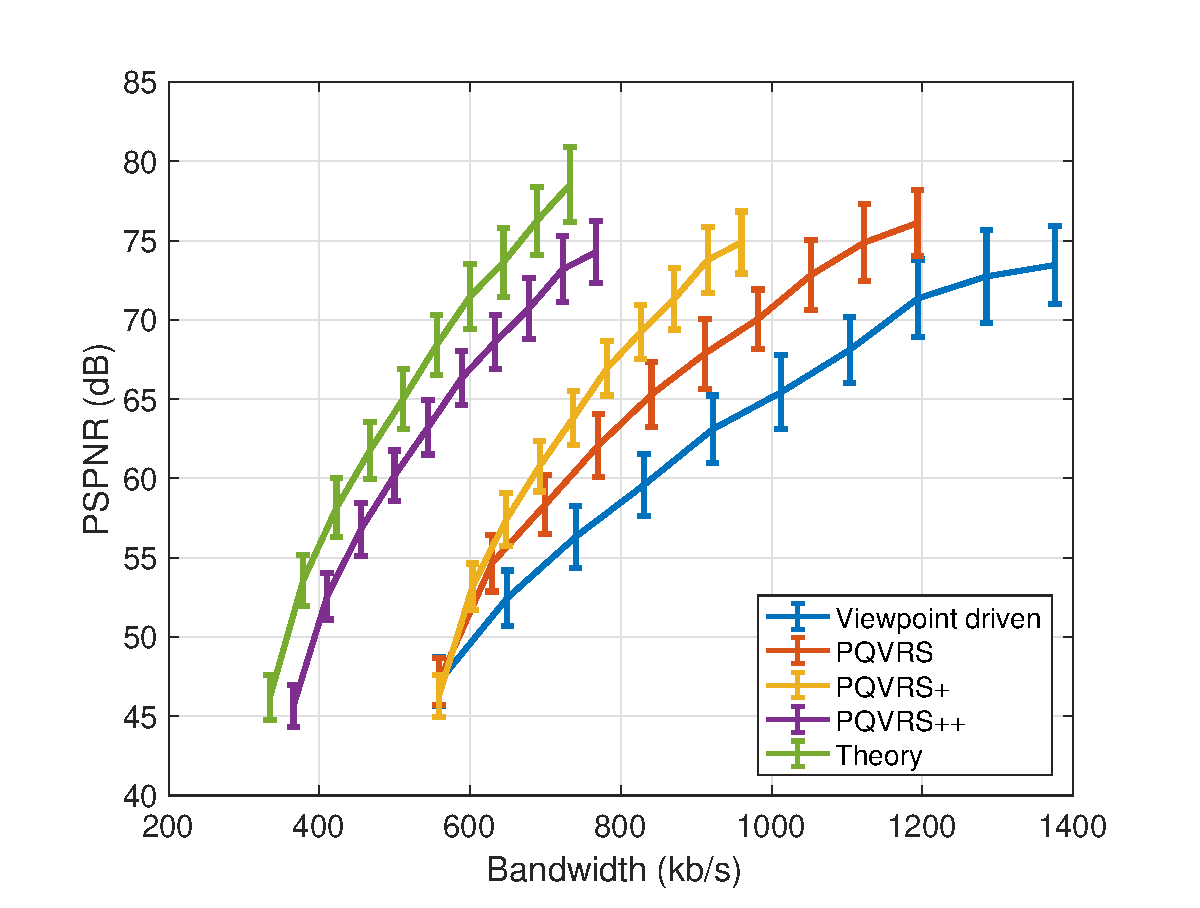
\includegraphics[width=3in]{images/practical_improvement.eps}
  \caption{PSPNR-bandwidth tradeoff of 5 methods: Viewpoint-driven, PQVRS, PQVRS+, PQVRS++, theoretical performance.}
  \label{practical_imp}
  \end{figure}

\subsubsection{Performance comparison under real-world bandwidth}

Actually, in real-world video streaming, bandwidth is unstable which may change significantly in a short time. When the bandwidth change dramatically from a high level to a low level, it not only decrease the value of PSPNR, but also causes stalling in video display, which is another important metric of perceived quality.

We test the performance of Flare and proposed PQVRS under the network with 800 kb/s bandwidth on average, but with different levels of bandwidth fluctuation. 

   \begin{figure}
  \centering
  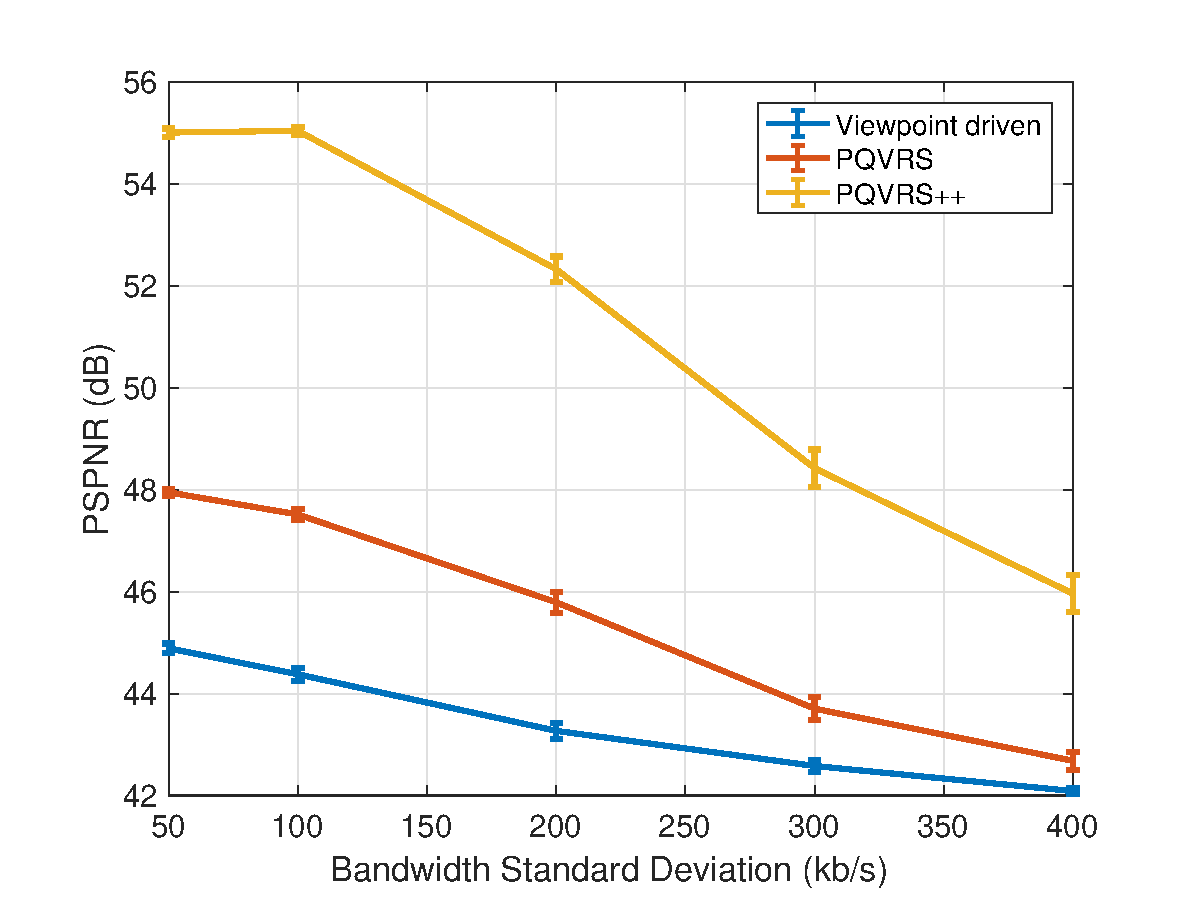
\includegraphics[width=3in]{images/throughput-PSPNR.eps}
  \caption{PSPNR of 5 methods: Viewpoint-driven, PQVRS, PQVRS+, PQVRS++, theoretical performance.}
  \label{practical_PSPNR}
  \end{figure}
  
    \begin{figure}
  \centering
  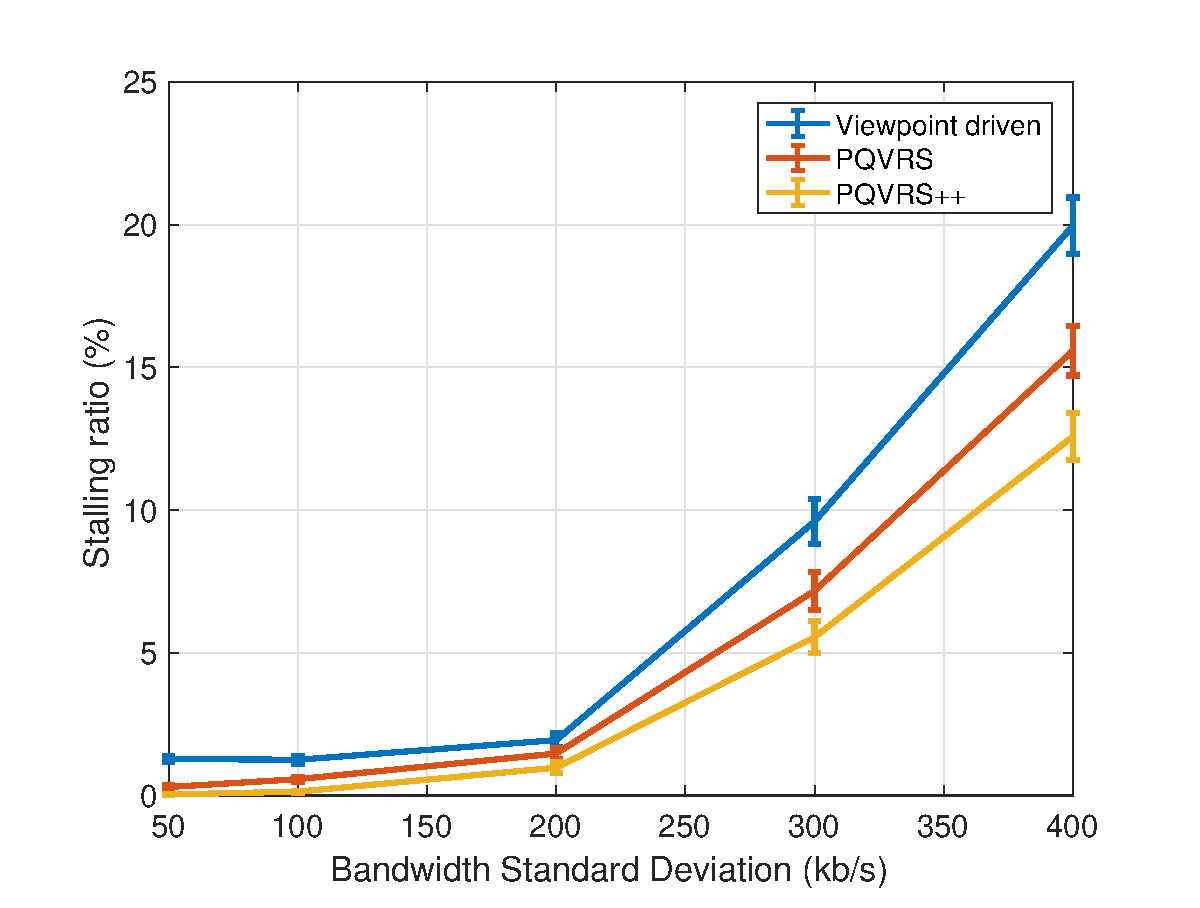
\includegraphics[width=3in]{images/throughput-stalltime.eps}
  \caption{Stalling of 5 methods: Viewpoint-driven, PQVRS, PQVRS+, PQVRS++, theoretical performance.}
  \label{practical_stall}
  \end{figure}

Fig. \ref{practical_PSPNR} presents average PSPNR of 3 methods, and Fig. \ref{practical_stall} presents average time of stalling of 3 methods.Result show that PQVRS++ improves 10 higher PSPNR and decreases 50\% stalling.

\subsection{Performance robustness under random user behavior}

In VR streaming, any system which takes advantage of viewpoint prediction or other user behavior prediction, will definitely suffer from the risk of prediction error due to randomness of user behavior. Although in most cases, user behavior (viewpoint, speed) is predictable, however, when user behavior is unpredictable, a robust streaming system should also present an acceptable performance, which will not give user a seriously bad perceived quality.

We generate a database of randomly moving user viewpoint, with different average moving speed. In our generated database, user's viewpoint is moving with a random speed to a random direction in each second, so it is completely unpredictable. Fig. \ref{random_improvement} shows our improvement compared with Viewpoint-driven method on these viewpoint traces.

    \begin{figure}
  \centering
  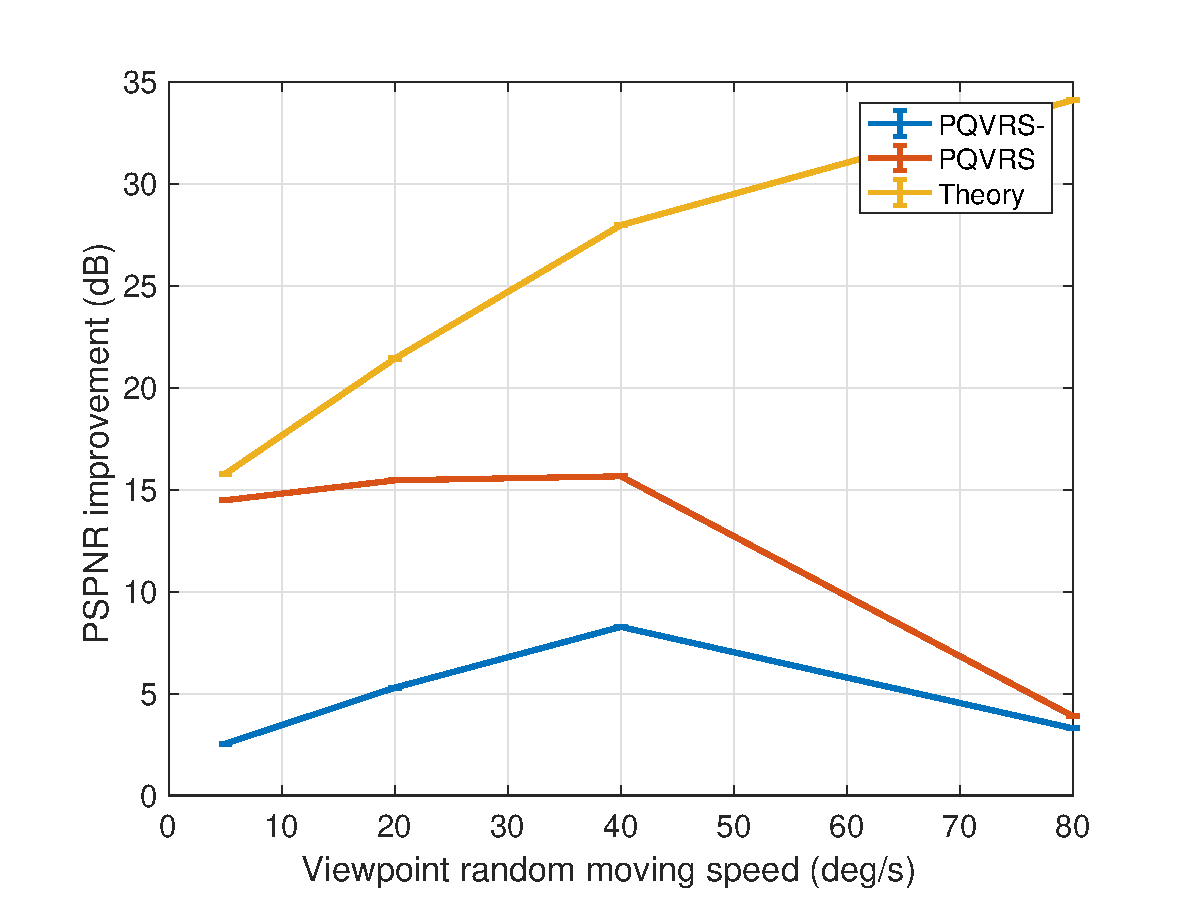
\includegraphics[width=3in]{images/random_improvement.eps}
  \caption{PSPNR improvement of PQVRS, PQVRS+, PQVRS++ and theoretical cases on random viewpoint traces, compared with viewpoint-driven VR streaming.}
  \label{random_improvement}
  \end{figure}

In this random, unpredictable user behavior, when viewpoint moving speed is below 20 deg/s, PQVRS++ can still reach a good improvement. Of course, in the worst case, when the speed get large enough, the predicted viewport will be totally wrong. PQVRS++ has nearly no improvement compared with viewpoint driven VR streaming since they both allocate high video quality on absolutely wrong place. But Fig. \ref{random_improvement} shows that in any case, PQVRS++ does not perform poorly than it.

\subsection{Real-world end-to-end experiment}

In this paper, we build our new JND model to compute PSPNR and use it as the metric to measure user-perceived quality. Now we prove PSPNR computed by our JND model can reflect user's rating for VR video display. We carry out real-world experiments of 21 different videos with different PSPNR displayed by Pano system. Each video is watched by 25 subjects and given the quality rating. Rating rule is shown in Fig. \ref{rating_rules}. Fig. \ref{pspnr_mos} scatters the average user rating of these 21 videos. We do a linear regression on these data and result shows that PSPNR and user rating has strong positive correlation. (correlation coefficient = 0.73)

    \begin{figure}
  \centering
  \includegraphics[width=3in]{images/rating.jpg}
  \caption{User rating rules.}
  \label{rating_rules}
  \end{figure}

    \begin{figure}
  \centering
  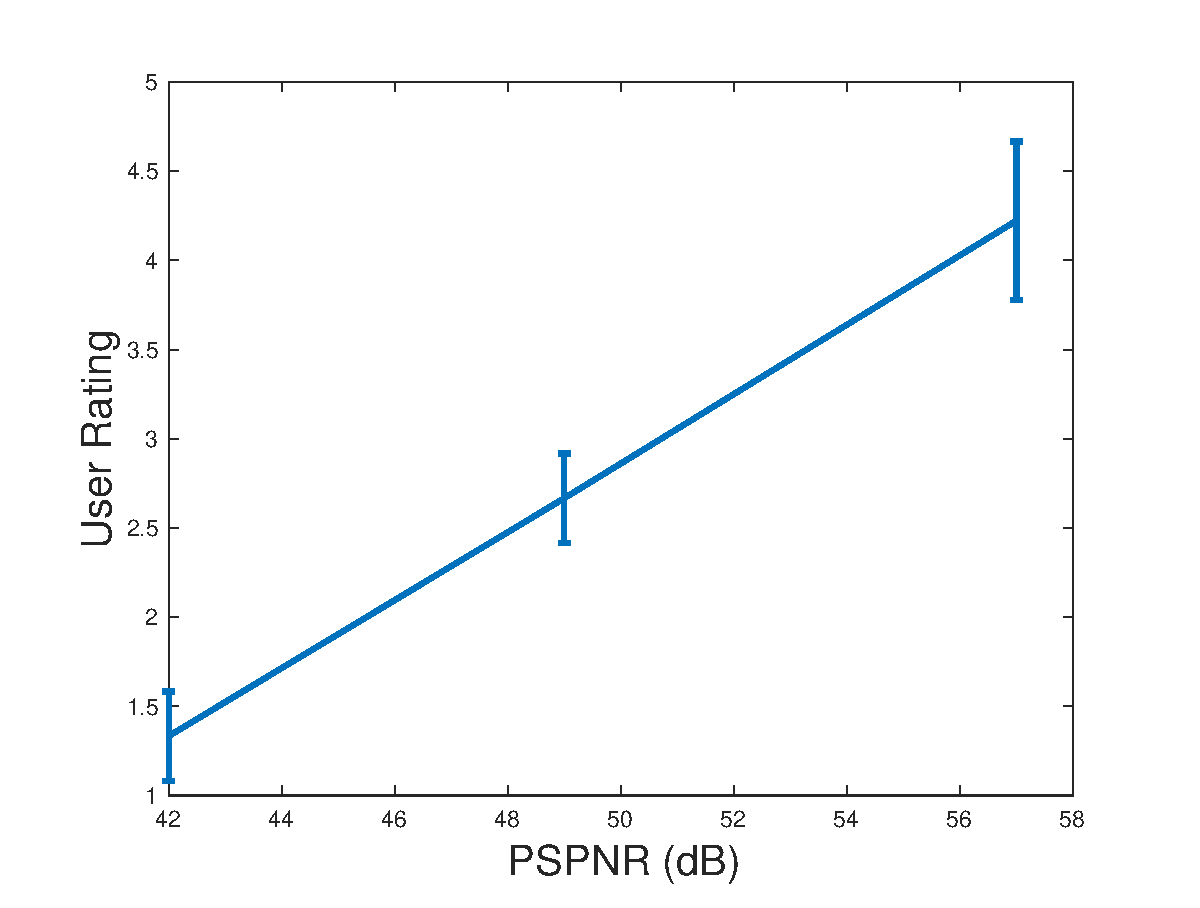
\includegraphics[width=3in]{images/pspnr_mos.eps}
  \caption{Relativity study of PSPNR and user rating. Each spot indicates average rating of one video from 25 different subjects.}
  \label{pspnr_mos}
  \end{figure}

Then we set up real-world end-to-end performance comparison between Flare, PQVRS and PQVRS++. 25 subjects participated in the experiments. For each subject, we shown him (her) a same VR video which is streaming by Viewpoint-driven, PQVRS and PQVRS++ in the same network condition. The order of display by 3 methods is random. After 3 displays, the subject give a rating of perceived quality for the three. Fig. \ref{rating_res} presents the result of user rating. Proposed PQVRS++ obtains score 3.35 on average, while PQVRS gets 2.8 and Flare gets only 1.8.

    \begin{figure}
  \centering
  \includegraphics[width=3in]{images/rating_result.png}
  \caption{User rating results.}
  \label{rating_res}
  \end{figure}

\subsection{Analysis of VR streaming workload}

We implement a prototype of Flare, PQVRS, and test their workload on Dell Precision 7920, to make comparison with proposed PQVRS++.

First we test client-side CPU workload. Although Dell Precision 7920 is a work station with 40 CPUs, now we only make 1 of them available, in order to simulate the performance on normal VR devices. Fig. \ref{CPUclient} shows the comparison of client-side CPU occupancy rate between Flare, PQVRS and PQVRS++, when streaming a 2880*1440 VR video for 1 minute duration. We notice that 85\% CPU workload comes from video decoding \& rendering, and content downloading, perceived quality computation and quality allocation in PQVRS introduce negligible CPU workload. In total, PQVRS++ saves 5\% CPU workload compared with Flare. This marginal benefit is mainly because we decreases the number of tiles need to be decoded by clients per segment, which makes decoder a bit faster. (as described in \S 7)

    \begin{figure}
  \centering
  \includegraphics[width=3in]{images/CPUworkload.eps}
  \caption{Client-side CPU workload comparison between Flare, PQVRS and PQVRS++.}
  \label{CPUclient}
  \end{figure}
  
Server-side workload comparison is done with all 40 CPU available. Result is shown in Fig. \ref{CPUserver}. Since all modules on server-side are offline works, we test the CPU processing time for each single 1-minute VR video, rather than CPU occupancy rate. Results show that the dominant part of server-side processing time is video encoding. The processing time of PSPNR computation is negligible. So PQVRS++ doesn't introduce considerable workload for video server.

    \begin{figure}
  \centering
  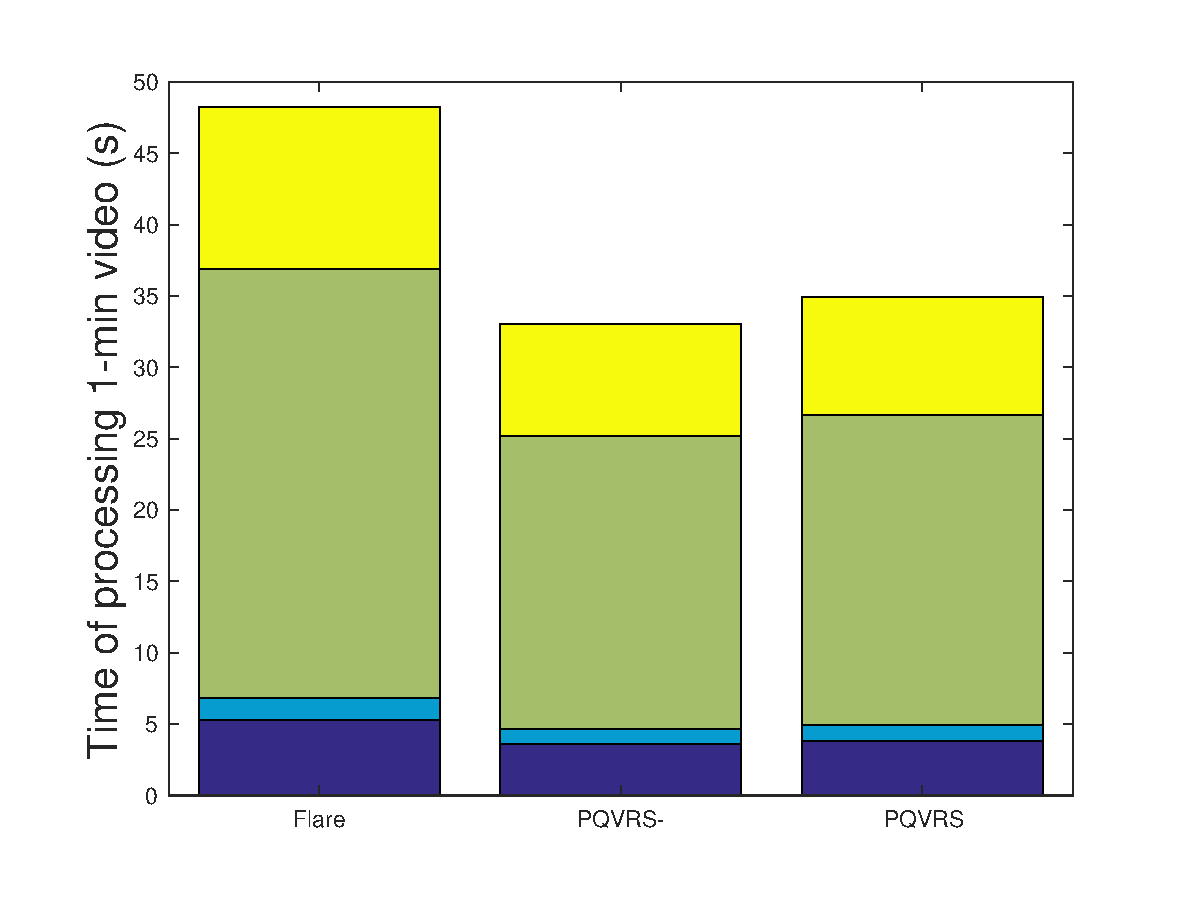
\includegraphics[width=3in]{images/Processtime.eps}
  \caption{Server-side CPU workload comparison between Flare, PQVRS and PQVRS++.}
  \label{CPUserver}
  \end{figure}